\documentclass{beamer}
\usetheme{Madrid}
\usepackage[T1]{fontenc}
\usepackage{mathpazo}
\usepackage{graphicx}
\usepackage{booktabs}
\usepackage{tikz}
\usetikzlibrary{positioning,arrows.meta,shapes.geometric,fit,backgrounds,calc}
\definecolor{cetnavy}{RGB}{10,26,63}
\definecolor{cetlight}{RGB}{225,231,242}
\setbeamercolor{structure}{fg=cetnavy}
\setbeamercolor{frametitle}{bg=cetnavy,fg=white}
\setbeamercolor{title}{bg=cetnavy,fg=white}
\setbeamertemplate{navigation symbols}{}
% =====================================================================
%  EDIT YOUR DETAILS HERE — this ONE file feeds every abstract & deck.
%  (Change a value, recompile; all 36 documents update.)
% =====================================================================
\newcommand{\seminarName}{Aflah Muhammed P}      % <-- your full name (guessed from your email; please verify)
\newcommand{\seminarRoll}{TVE00CS000}            % <-- your university register/roll number
\newcommand{\seminarClassRoll}{00}               % <-- your class roll no (the short one)
\newcommand{\seminarGuide}{Prof.\ <Guide Name>}  % <-- your guide
\newcommand{\seminarDept}{Department of Computer Science and Engineering}
\newcommand{\seminarCollege}{College of Engineering Trivandrum}
\newcommand{\seminarShortCollege}{CET}           % shown in the slide footer, e.g. "Aflah Muhammed P (CET)"
\newcommand{\seminarShortTitle}{B.Tech Seminar}  % middle of the slide footer
\newcommand{\seminarDate}{July 31, 2026}
% ---------------------------------------------------------------------
% Optional: put a logo image named  cet_logo.png  in this folder and it
% will appear on every title slide automatically. If absent, it is skipped.
% =====================================================================

\title[\seminarShortTitle]{Model Context Protocol: Landscape, Security Threats, and Directions}
\author[\seminarName\ (\seminarShortCollege)]{\seminarName \\ \seminarRoll \\ Roll No: \seminarClassRoll \\ Guide: \seminarGuide}
\institute[\seminarShortCollege]{\seminarDept \\ \seminarCollege}
\date{\seminarDate}
\titlegraphic{\IfFileExists{cet_logo.png}{\includegraphics[height=1.1cm]{cet_logo.png}}{}}
\begin{document}
\begin{frame}\titlepage\end{frame}
\begin{frame}{Table of Contents}\tableofcontents\end{frame}
\section{Introduction}
\begin{frame}{What is the Model Context Protocol?}
\textbf{\textit{An open standard for tool-augmented AI}}
\begin{itemize}
  \item Introduced by Anthropic in late 2024.
  \item Often called the ``USB-C port for AI applications.''
  \item Unified, bidirectional protocol between LLMs and tools.
  \item Enables dynamic discovery of external tools and data.
  \item Replaces bespoke, one-off integration connectors.
\end{itemize}
\end{frame}

\begin{frame}{Why security matters now}
\begin{itemize}
  \item Adoption is rapid and community-driven.
  \item Servers execute largely untrusted code.
  \item Tool descriptions are implicitly trusted by the model.
  \item Marketplaces are loosely curated.
  \item Security study has lagged behind deployment.
\end{itemize}
\end{frame}

\section{Literature Survey}
\begin{frame}{Related work and context}
\begin{itemize}
  \item Function-calling and plugin ecosystems (OpenAI, LangChain).
  \item Prompt-injection studies on tool-augmented agents.
  \item MCP Safety Audit: automated server scanning (2025).
  \item Agent sandboxing and least-privilege execution.
  \item This paper: first systematic MCP-focused survey.
\end{itemize}
\end{frame}

\section{Motivation}
\begin{frame}{Motivation}
\begin{itemize}
  \item MCP is becoming core agent infrastructure.
  \item Tens of thousands of servers across many marketplaces.
  \item Adopters span IDEs, clouds, and financial services.
  \item No unified view of its attack surface exists.
  \item A shared threat vocabulary is urgently needed.
\end{itemize}
\end{frame}

\section{Problem Statement}
\begin{frame}{Problem Statement}
\begin{itemize}
  \item MCP lacks a systematic security characterisation.
  \item Trust boundaries between host, server, and data are unclear.
  \item Malicious or drifting servers can silently harm users.
  \item Threats span the entire server lifecycle.
  \item Safeguards are ad hoc and phase-agnostic.
\end{itemize}
\end{frame}

\section{Objectives}
\begin{frame}{Objectives and Contributions}
\begin{itemize}
  \item Formalise the MCP architecture and components.
  \item Define a four-phase server lifecycle (16 activities).
  \item Build a taxonomy of 16 threat scenarios.
  \item Group threats under four attacker types.
  \item Recommend lifecycle-specific safeguards.
\end{itemize}
\end{frame}

\section{Methodology Overview}
\begin{frame}{Methodology Overview}
\begin{center}
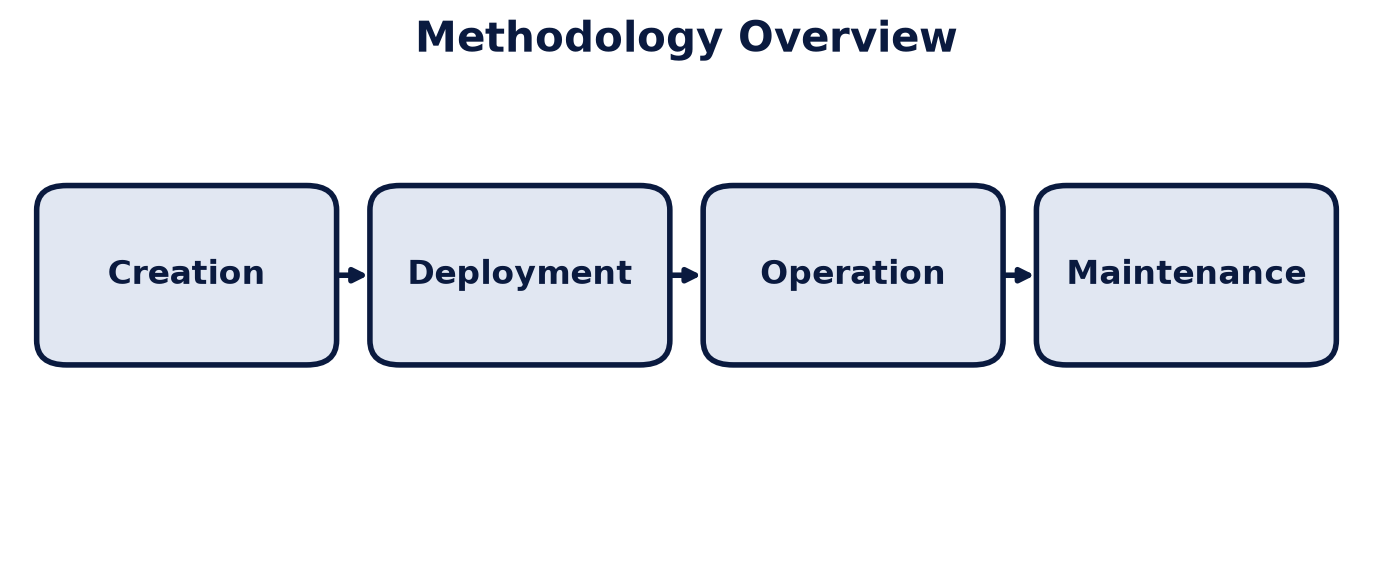
\includegraphics[width=0.9\textwidth,height=0.62\textheight,keepaspectratio]{images/mcp_1.png}
\end{center}
\vspace{2mm}
\begin{center}\small Threats are mapped to each phase of the MCP server lifecycle.\end{center}
\end{frame}

\section{System Architecture}
\begin{frame}{MCP Architecture}
\begin{center}
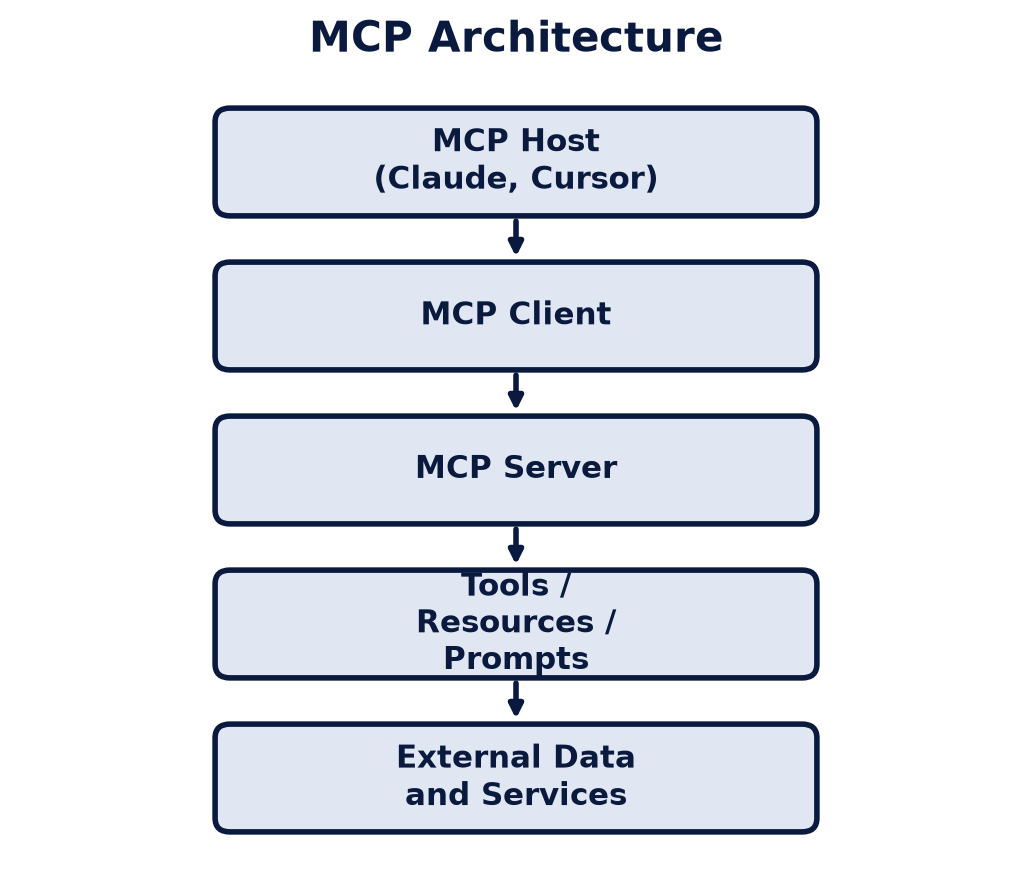
\includegraphics[width=0.9\textwidth,height=0.62\textheight,keepaspectratio]{images/mcp_2.png}
\end{center}
\end{frame}

\begin{frame}{Component roles}
\begin{itemize}
  \item \textbf{Host}: AI app orchestrating tool use.
  \item \textbf{Client}: one-to-one link managing requests.
  \item \textbf{Server}: exposes tools, resources, and prompts.
  \item \textbf{Transport}: bidirectional, notification-driven channel.
\end{itemize}
\end{frame}

\section{Data Collection}
\begin{frame}{Scope and Sources}
\begin{itemize}
  \item Survey of the live MCP ecosystem.
  \item Servers indexed across dozens of marketplaces.
  \item Sources: MCP.so, Smithery, Glama, PulseMCP.
  \item Curation is inconsistent; some listings mis-categorised.
  \item Data released publicly for community verification.
\end{itemize}
\end{frame}

\section{Model Development}
\begin{frame}{Threat Taxonomy}
\begin{center}
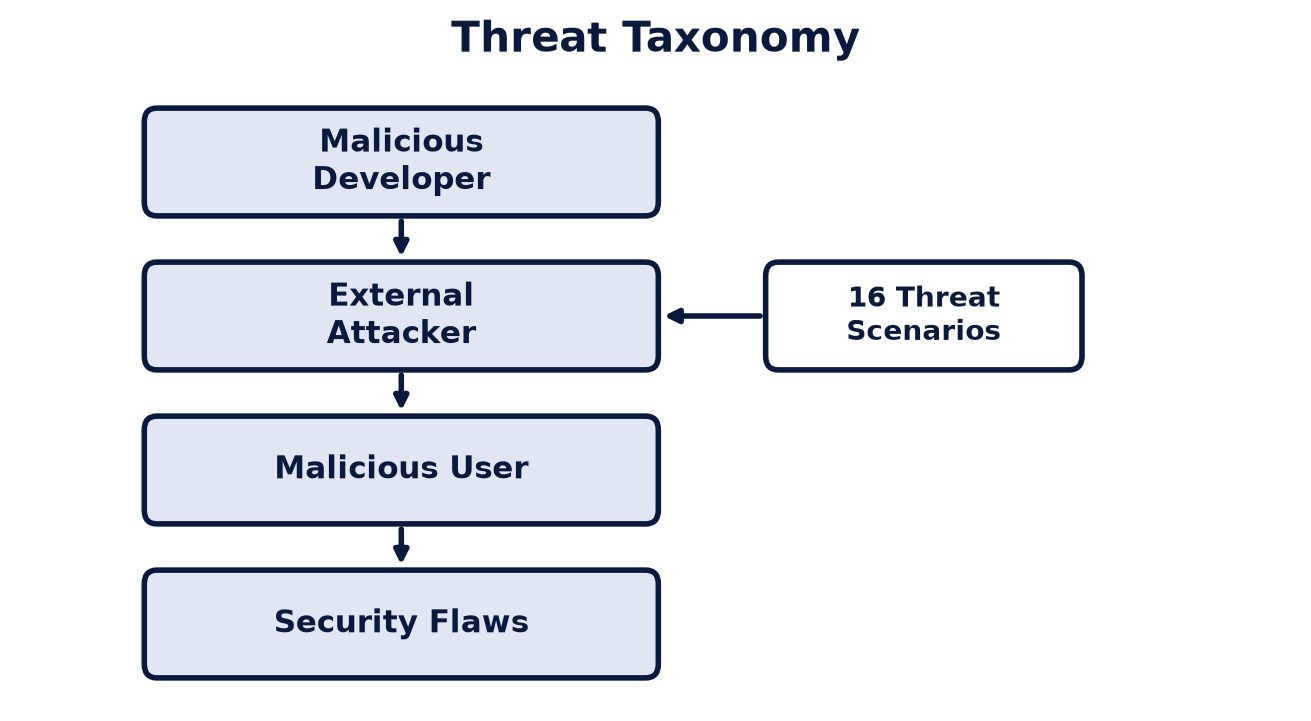
\includegraphics[width=0.9\textwidth,height=0.62\textheight,keepaspectratio]{images/mcp_3.png}
\end{center}
\end{frame}

\begin{frame}{Representative attacks}
\begin{itemize}
  \item \textbf{Tool poisoning}: hidden logic exfiltrates SSH keys.
  \item \textbf{Rug pull}: trusted server later adds a backdoor.
  \item \textbf{Cross-server shadowing}: intercepts another tool's data.
  \item \textbf{Indirect prompt injection}: instructions hidden in resources.
  \item \textbf{Typosquatting}: deceptively similar server names.
\end{itemize}
\end{frame}

\section{Results}
\begin{frame}{Lifecycle threats and safeguards}
\footnotesize
\begin{center}
\begin{tabular}{@{}lll@{}}
\toprule
\textbf{Phase} & \textbf{Example threat} & \textbf{Safeguard} \\
\midrule
Creation    & Tool poisoning        & Signed manifests \\
Deployment  & Installer spoofing    & Checksum verify \\
Operation   & Prompt injection      & Anomaly detection \\
Maintenance & Config. drift         & Reproducible builds \\
\bottomrule
\end{tabular}
\end{center}
\vspace{2mm}
\begin{center}\small 16 threats mapped across four lifecycle phases and attacker types.\end{center}
\end{frame}

\section{Discussions}
\begin{frame}{Discussion}
\begin{itemize}
  \item Model trust in tool descriptions is the core weakness.
  \item Openness and security are in tension.
  \item Attacks exploit missing identity and provenance.
  \item Defences must be aligned to lifecycle phases.
  \item No single layer suffices; defence must be layered.
\end{itemize}
\end{frame}

\section{Challenges}
\begin{frame}{Challenges and Limitations}
\begin{itemize}
  \item Weak trust boundaries and namespace governance.
  \item Verification overhead versus rapid growth.
  \item Proprietary platforms resist open data access.
  \item Specification lacks strong security primitives.
  \item Quality curation of marketplaces is immature.
\end{itemize}
\end{frame}

\section{Future Work}
\begin{frame}{Future Research Directions}
\begin{itemize}
  \item Federated or centralised namespace governance.
  \item Standardised authentication and capability negotiation.
  \item Automated server auditing and sandboxing.
  \item Transparent, reproducible update mechanisms.
  \item Sustainable, quality-driven ecosystem curation.
\end{itemize}
\end{frame}

\section{Conclusion}
\begin{frame}{Conclusion}
\begin{itemize}
  \item MCP standardises how LLM agents reach tools.
  \item First systematic map of its security landscape.
  \item Four-phase lifecycle, 16 threats, four attacker types.
  \item Lifecycle-specific safeguards are proposed.
  \item Trust and standardisation remain open problems.
\end{itemize}
\end{frame}

\section{References}
\begin{frame}{References}
\footnotesize
\begin{itemize}
  \item X. Hou, Y. Zhao, S. Wang, and H. Wang, ``Model Context Protocol (MCP): Landscape, Security Threats, and Future Research Directions,'' arXiv:2503.23278, 2025.
  \item Anthropic, ``Introducing the Model Context Protocol,'' 2024.
  \item B. Radosevich and J. T. Halloran, ``MCP Safety Audit: LLMs with the Model Context Protocol Allow Major Security Exploits,'' arXiv:2504.03767, 2025.
\end{itemize}
\end{frame}
\begin{frame}\vfill\centering{\Huge Thank You}\vfill\end{frame}
\end{document}
